\documentclass[12pt,a4paper]{article}
\synctex=1
\usepackage[utf8]{inputenc}
\usepackage[margin=1cm]{geometry}
\usepackage{graphicx}
%\usepackage{verbatim}
\usepackage{amsmath}
\usepackage{amsfonts}
\usepackage{amssymb}
\usepackage{listings}
\usepackage{enumitem}
\usepackage{textcomp}
\usepackage{courier}
\usepackage{libertine}
\usepackage{pgfornament}
\usepackage{eso-pic}
\usepackage[hangul]{kotex}
\linespread{1.3}

\title{
	\centering
	\pgfornament[width=12cm,color=teal]{84}\\
	\vspace{1cm}
	\fontsize{50}{50} \selectfont {정보통신 수학 및 실습\\Homework}\\
		\pgfornament[width=12cm,color=teal]{88}\\
	\vfill}
\author{
	\LARGE
	\begin{tabular}{rl}
		\hline
		학번 : & 2016110056\\ 
		학과 : & 불교학부 \\
		이름 : & 박승원\\
		날짜 : & \today\\
		\hline
	\end{tabular}\vspace{2cm}
	\\

\includegraphics[width=0.5\textwidth]{logo.jpg}
	}
\date{}


\begin{document}
\maketitle
\pagenumbering{gobble}
\noindent
\lstset{language=matlab, columns=flexible, tabsize=4, frame=shadowbox, showstringspaces=false, breaklines=true, upquote=true, basicstyle=\normalsize}

\renewcommand{\thesubsubsection}{\alph{subsubsection})}
\renewcommand{\thesubsection}{\arabic{subsection}.}
\newpage
\section*{Chapter 3 Homework}

\subsection{Simplify the following equations.}

\subsubsection{$\cos(100\pi t)\cos(500\pi t) = \dfrac{\cos(600\pi t)+\cos(400\pi t)}{2}$}
$e^{i\theta} = \cos\theta + i\sin\theta\\
e^{i\alpha} \times e^{i\beta} = (\cos\alpha + i\sin\alpha)(\cos\beta+i\sin\beta)\\
e^{i(\alpha + \beta)} = \cos\alpha\cos\beta-\sin\alpha\sin\beta + i(\sin\alpha\cos\beta+\cos\alpha\sin\beta)=\cos(\alpha+\beta) + i\sin(\alpha+\beta)\\
\therefore \cos(\alpha+\beta) = \cos\alpha\cos\beta -\sin\alpha\sin\beta\\
\sin(\alpha+\beta) = \sin\alpha\cos\beta+\cos\alpha\sin\beta\\
\cos(\alpha-\beta) = \cos\alpha\cos\beta +\sin\alpha\sin\beta\\
\sin(\alpha-\beta) = \sin\alpha\cos\beta-\cos\alpha\sin\beta\\
\therefore \cos(\alpha+\beta) + \cos(\alpha-\beta)= 2\cos\alpha\cos\beta\\
\cos\alpha\cos\beta = \dfrac{\cos(\alpha+\beta)+\cos(\alpha-\beta)}{2}\\
\sin\alpha\cos\beta = \dfrac{\sin(\alpha+\beta)+\sin(\alpha-\beta)}{2}$
\subsubsection{$4sin(200\pi t)cos(300\pi t)=-2\sin(500\pi t
	)\sin(100\pi t)$} 

\subsection{Find the frequency of the following signals.} 
\subsubsection{$\sin(t)$}
$2\pi f = 1\\ 
\therefore f = \dfrac{1}{2\pi}$
\subsubsection{$\cos(600\pi t)$}
$2\pi f = 600\pi\\
\therefore f =  300$

\subsection{Evaluate the following functions.} 
\subsubsection{$sin(\pi /4)$}
$\dfrac{\sqrt{2}}{2} $
\subsubsection{$tan(\pi )$} 
0
\subsection{Let the information signal $m(t)=4\sin (200\pi t)$ \\
	and the carrier signal $c(t)=\cos(2\times 10^6\pi t)$.\\
Simplify the transmission signal $x(t)=m(t)c(t)$ and	find its frequencies. \\
 Plot the magnitude of each frequency in the	frequency domain.} 
$x(t) = 4\sin(200\pi t)\cos(2\times 10^6\pi t)=2(\sin(2\times 10^6\pi + 200\pi )t)+\sin(2\times 10^6\pi - 200\pi) t))\\
\therefore f = 10^6 \pm 100$

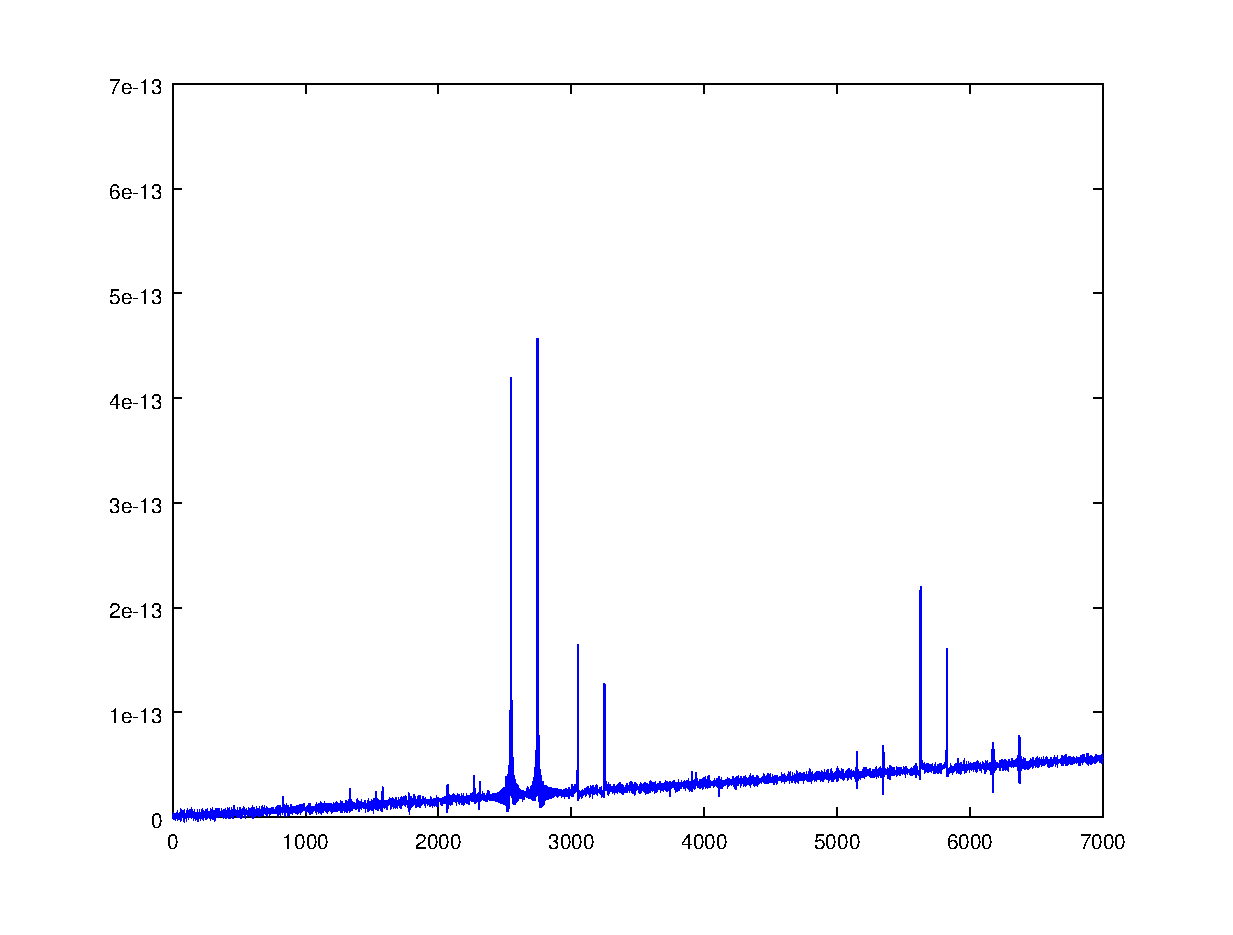
\includegraphics[width=0.8\textwidth]{h.eps}

\end{document}
